{\textbf{1. 传输介质的分类}}

{传输介质分为两大类:}{\textbf{{导向性传输介质}}(如双绞线和光纤)和\textbf{{非导向性传输介质}}(如红外线、微波)。}

{\textbf{2. 双绞线}}

把两根互相绝缘的铜导线绞合起来。其特点是既可以传输模拟信号,又可以传输数字信号。{双绞线又可分为}\textbf{{无屏蔽双绞线和屏蔽双绞线}}{。屏蔽双绞线就是在普通的双绞线外加上金属丝编织的屏蔽层,以起到提高抗电磁干扰的能力,如图2-8所示。}

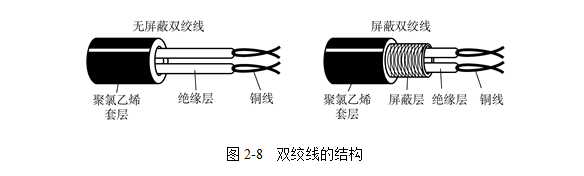
\includegraphics[width=4.00000in,height=1.20833in]{png-jpeg-pics/83D05E79CEEF97DB4600E5A2E01AF609.png}

\textbf{{3. 同轴电缆}}

由内导体铜质芯线、绝缘层、网状编织的外导体屏蔽层以及保护塑料外层组成。它比双绞线的抗干扰能力强,因此传输距离更远。如图2-9所示。

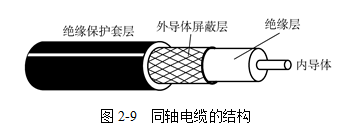
\includegraphics[width=2.75000in,height=1.05208in]{png-jpeg-pics/1D1DB4FC651BA5851336A50535D58EA2.png}

\textbf{{4. 光纤}}

即光导纤维,根据光线传输方式不同,光纤可分为\textbf{单模光纤和多模光纤}。其主要优点是频带宽、衰减小、速率高、体积小、抗雷电和电磁干扰性好、误码率低、质量轻、保密性好等。

\textbf{单模光纤:}直径只有一个光波的波长,光线在其中一直向前传播,不会发生多次反射,如图2-10所示。\textbf{单模光纤的光源使用的是昂贵的半导体激光器},而不使用较便宜的发光二极管,因此\textbf{单模光纤的衰减较小,适合远距离传输}。\\
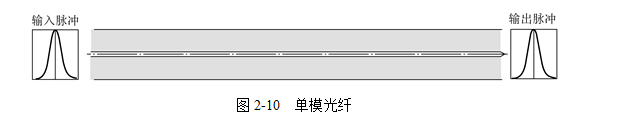
\includegraphics[width=3.35417in,height=0.66667in]{png-jpeg-pics/3F2AFE1999272C72B4C49C9C5C82E862.png}

\textbf{多模光纤:}利用光的全反射特性,如图2-11所示。\textbf{多模光纤的光源为发光二极管}。由于光脉冲在多模光纤中传输会逐渐展宽,造成失真,因此\textbf{多模光纤只适合近距离传输}。

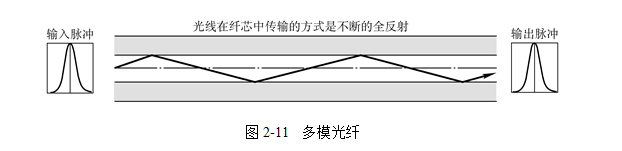
\includegraphics[width=3.35417in,height=0.81250in]{png-jpeg-pics/B3144BFA68F44A13A555A048CD9CFCBB.png}

\textbf{\textbf{{5. 非导向性传输介质}}\\
}

\textbf{非导向性传输介质}有短波、微波、红外线与可见光等。常见的通信方式有短波通信、微波通信、卫星通信、激光通信等。
